
\documentclass[proposal]{umassthesis}  
\usepackage{amsmath}
\usepackage{graphicx}
\usepackage{amsfonts}
\usepackage{algorithm}
\usepackage{algpseudocode}
\usepackage{multirow}
\usepackage{subfig}

\begin{document}

\title{Explorations into Machine Learning Techniques for Precipitation Nowcasting}

  
\author{Aditya Nagarajan}
\date{May 2016}
                     
\copyrightyear{2015}
\bachelors{B.E}{Madras Institute of Technology}
\masters{M.Sc.}{University of Massachusetts, Amherst}
\committeechair{David L. Pepyne}
\firstreader{Michael Zink}
\secondreader{Hari Balasubramanian}
\departmentchair[Professor and Department Head]{Sundar Krishnamurthy} 
\departmentname{Department of Mechanical and Industrial Engineering}

 \degree{Master of Science}{M.S.}

\frontmatter
\maketitle
\signaturepage

\chapter{Acknowledgments}             % Acknowledgements page
This work was performed within the UMass Center for Collaborative Adaptive Sensing of the Atmosphere (CASA) under funding provided by the Jerome M. Paros Endowment for Measurement Science Research.

\begin{abstract}

YOU SHOULD WRITE YOUR ABSTRACT TO LOOK MORE LIKE THE FIRST PART OF YOUR INTRODUCTION.

Weather surveillance radars are an excellent source of information for making real-time assessments and short-term predictions of rainfall - where it is occurring, its intensity, how much has accumulated so far, where it is moving, and so on. However they are limited in that, under normal operation, they can only sense active rainfall; they cannot sense the buildup and advection of the atmospheric water vapor commonly termed as  precipitable water which are the driving force behind severe storms. We thus explore this complimentary nature in the atmosphere that the build up of precipitable water which can potentially lead to precipitation. In this thesis we look at a novel way to predict short term (0-2 hours) precipitation commonly termed as nowcasting, by supplementing weather radar based reflectivity products with GPS derived Integrated Precipitable Water (IPW) vapor products derived from a network of GPS-Meteorology stations. We propose to develop a software system that computes point measurements of IPW from raw GPS signals and meteorological data from publicly available databases, to build spatial IPW fields and study its spatial and temporal properties with regard to evolving weather radar reflectivity fields. We explore the spatiotemporal relationship between IPW and reflectivity fields by analyzing severe storm events in the Dallas Fort-Worth region during the year of 2014. We then propose an approach involving state of the art machine learning and image processing techniques to develop a tool that takes sequences of gridded atmospheric IPW and radar reflectivity fields that predicts the future gridded rainfall field. We develop a nowcasting learning algorithm which takes spatiotemporal evolutions of IPW and reflectivity to predict the rainfall field one hour ahead. 

% We propose to build a software system to retrieve raw GPS signal data, associated surface meteorological data and radar reflectivity data from publicly available data sources, processing the data to produce spatial-temporal atmospheric water and rainfall information over the Dallas, Fort-Worth Texas region. Using this data the spatial and temporal patterns that atmospheric water exhibits before convective rainfall is analyzed for its potential to predict such events. We then propose an approach involving image processing and image-based machine-learning techniques to develop a tool that takes sequences of gridded atmospheric water fields and gridded weather radar fields and predicts the future gridded rainfall field.
\end{abstract}

\tableofcontents                % Table of contents
\listoftables                   % List of Tables
\listoffigures                  % List of Figures


\mainmatter   %% <-- This line is mandatory


\chapter{Introduction}

We live in an age where increasing volumes of different kinds of data are being made available in on-line databases in near real-time. Coupled with recent advances in big data technologies, particularly cloud computing and machine learning, a host of new tools have become available to rapidly process this data to obtain valuable insights and make actionable decisions from the data. One area particularly ripe for an application of these new big data technologies is environmental sensing, where by law the federal government is required to make the data from its many environmental sensor assets publicly available, which today means through on-line databases. Motivated by this, this thesis will explore the weather forecasting problem from a big data perspective.

Specifically, this thesis will seek to apply data science and machine-learning techniques to the problem of nowcasting (making short-term predictions) of precipitation fields 1-3 hours in the future from time-sequences of past spatial fields of precipitable water vapor and weather radar reflectivity. With precipitable water vapor a measure of the amount of water in the atmosphere that could potentially fall as rain and weather radar reflectivity a measure of falling rain, these two fields give information about the potential for rain and the active occurrence of rain in time and space. Using the complementary nature of these two measurements we will apply machine-learning techniques to analyze the spatiotemporal patterns and correlations between these two fields and then to use those patterns and correlations to make 1-3 hour precipitation nowcasts. In addition to the challenge of obtaining and pre-processing the input data for our analysis, we also face the challenge of developing machine learning algorithms that can handle spatiotemporal input data - essentially short video streams of precipitable water vapor and radar reflectivity fields to predict a video output for what the precipitation field will look like 1-3 hours in the future.

\section{Precipitation Nowcasting}

Because rain affects so many human activities, predicting rain has a long history. Whereas long-term rainfall forecasts (i.e., beyond 3 hours in the future) are based on models of atmospheric processes (cf. \cite{lynch2008origins}), short-term 1-3 hour nowcasts are frequently based on weather radar data. This is because numerical weather models tend to be too computationally time-consuming for real-time predictions. Nowcasts can be "manual" as when a weather radar meteorologist plays a radar reflectivity loop to infer where and how fast a storm is moving. Nowcasts can be automated as with the Storm Cell Identification and Tracking (SCIT) algorithm [ADD CITATION] uses the history radar data to identify storm cells and estimate their speed and direction or the Dynamic Adaptive Radar Tracking of Storms (DARTS) algorithm \cite{ruzanski2011casa} that uses the history of radar data to infer its rate of advection in order to project the reflectivity field 1-20 minutes into the future. Nowcasts based on weather radar data alone tend to quickly break down, so that a 20-minute DARTS nowcast of the reflectivity will often bear little resemblance to the actual reflectivity field that occurs 20 minutes in the future. This is because nowcast techniques based on weather radar data alone, while they can obtain a good estimate of storm advection, have very little skill in predicting storm growth and decay. They are thus very poor at predicting that a storm will pop-up at a given location when there is currently no radar data coming from that location, and they are very poor at recognizing that a storm will dissipate 20 minutes from now when it is currently growing in intensity. This has lead many to look for other information with which to augment weather radar data.

Since the discovery in the early 1990s that GPS signal propagation delays can be used to infer atmospheric water vapor content \cite{bevis1992gps} \cite{bevis1994gps} there has been significant maturation in GPS-Meteorology (GPS-Met) technology and techniques. NOAA (National Oceanic and Atmospheric Administration), UCAR (University Collaboration of Atmospheric Research) and SOPAC (Scripps Orbital and Permanent Array Center) have contributed to the development, operation and maintenance of a nationwide realtime GPS-based water vapor monitoring system \cite{wolfe2000developing} \cite{bock1997scripps}. This has lead to the availability of real-time water vapor products to the public and operational forecasters from over 500 GPS-Met stations distributed around the continental United States. In addition, it is also possible to obtain mature, validated software for GPS-Met calculations (e.g., [CITE GAMIT]) allowing for research deployments of GPS-Met stations [CITE ADITYA AMS PAPER] and repurposing of GIS Continuously Operating GPS Reference Stations (CORS http://geodesy.noaa.gov/CORS/) stations for the GPS-met application.

Motivated by the fact that in the water cycle that describes the movement of water through the atmosphere, water must first exist in the atmosphere as water vapor before it becomes rain, a number of agencies and researchers have explored the potential of real-time observations of atmospheric water vapor content derived from GPS-Met stations for weather forecasting and precipitation nowcasting. Japan thus far has the highest density of GPS stations with an average spacing between stations of 17km \cite{shoji2014estimation}. Using this densely spaced GPS network, a number of studies have looked into the ability of high spatial-temporal resolution GPS-Met derived Integrated Precipitable Water Vapor (IPW) to nowcast thunderstorms and severe rain, e.g., \cite{iwasaki2002diurnal}, \cite{seko2004meso}. In a study of how IPW fields relate to the onset convective weather \cite{inoue2007characteristics} showed that the maximum IPW occurred 1-2 hours prior to thunderstorm activity where thunderstorms were measured using cloud-to-ground lightning and convective activity was measured by hourly accumulated rainfall. In another study looking at relationships between spatial variations in IPW and precipitation it was shown that rainfall intensity is related to IPW gradients and in particular that strong convergence (concentration) of water vapor is generally present several hours in advance of convective precipitation \cite{yoshinori2013retrieval}.

Spatial variations in IPW and their correlations with thunderstorm activity have also been studied in Europe. De Haan \cite{de2009real} devised a method to construct IPW maps from a network of GPS stations using two dimensional variational techniques. The IPW maps were then studied with regard to lightning and thunderstorm events in the Netherlands. The level of convergence of water vapor evident in the IPW fields again correlated well with subsequent precipitation rates and thunderstorm activity. A similar analysis was conducted in Spain \cite{terradellas2010use} using normalized IPW fields to take into account the seasonal variation. The interesting observation made in this paper is that the decay of IPW values coincided with storm direction and intensity.

Generation and validation of IPW fields has also been carried in the US for its potential for analyzing long- and short-term climatological activity \cite{radhakrishna2015precipitable}, \cite{shi2015real},  \cite{akilan2015gps}. As with the work in Japan and Europe, it was again observed that IPW usually peaks a few hours to the onset of precipitation and the variations in IPW and the variations of rainfall rate are also strongly correlated. However \cite{shi2015real} and \cite{akilan2015gps} both also note that IPW alone can not be used as an indicator of rainfall and there are other atmospheric parameters that play a role in the onset of rain. This observation is based on peak IPW values encountered at times which did not follow up with any rainfall.

Based on the above findings, we propose a precipitation nowcasting approach that uses both IPW and weather radar reflectivity. Rather than attempting a prediction system that tries to model how these to fields jointly evolve, we propose instead a machine learning approach to learn the joint spatial-temporal patterns and correlations.

The use of machine learning in precipitation nowcasting is not new. An early application of machine learning to the precipitation nowcasting problem used artificial neural networks to predict rainfall fields 1 hour in advance based on the current rainfall field \cite{french1992rainfall}. A single layer neural network was trained using a $100 \times 100 km^{2}$ domain, 4 km resolution precipitation field to predict the corresponding precipitation field 1 hour in the future. The predictions were evaluated against mean areal index (MAI) and PAC (Percent Areal Coverage) and performed as well as the standard nowcasting algorithm of the time. A neural network approach was also applied to forecasting rain gauge readings with 0-6 hr lead times using moisture and updraft data from the NCEP (National Center for Environmental prediction) Nested Grid Point Model. A feature selection method was used to reduce the initial 528 feature input space to the 25 most important features \cite{kuligowski1998localized}.

Machine learning approaches that combine large numbers of weather variables include \cite{mecikalski2015probabilistic} where GOES satellite cloud data along with NWP (numerical weather prediction) data was used to determine probabilistic estimates of convective storms and turbulence 1 hour in advance. The learning problem addressed used random forest and logistic regression classifiers to determine if a particular cloud would turn into a convective storm. The random forest algorithm was a special kind, called the Spatiotemporal Relational Random Forest (SRRF) \cite{mcgovern2010understanding}, developed for data sets which contain spatiotemporal features, in this case cloud imagery.  Using the ability of the random forest to provide measures of feature importance they showed how augmenting GOES satellite data with various NWP model parameters could improve the accuracy of the nowcasts.

The state-of-the-art machine learning algorithms of today fall under the category of "Deep Learning" \cite{arel2010deep}. The word "Deep" is coined here to emphasize the fact that this type of learning algorithm tries to learn multiple layers of representations of the input data space. These multiple layers of representations take advantage of the spatial correlations of an input image or the temporal correlations of time series time series data. Some of the well known deep learning architectures include Convolutional Neural Networks (CNN), Recurrent Neural Networks (RNN) and LSTM (Long Short Term Memory). A very recent application of Deep Learning and one of the first in the meteorological domain to tackle the nowcasting problem used a CNN-LSTM, an combination of Convolution and LSTM, to predict rainfall fields based on spatiotemporal sequences of radar reflectivity products \cite{shi2015convolutional}. They develop a CNN-LSTM deep neural network architecture to predict 15 frames of radar reflectivity echoes from the previous 5 frames of reflectivity. The algorithm was trained and tested on a dataset of reflectivity echoes from a radar in Hong-Kong for rainfall days which occurred over a period of three years. The results showed that the CNN-LSTM performs better than the current model based state-of-the-art nowcasting algorithm called the Real-time Optical flow by Variational methods for Echoes of Radar (ROVER). 

In this thesis we attempt to go a step beyond the above work (the first which uses only reflectivity, the second which relies on NWP data, and the third, which again uses only reflectivity), to develop an automated precipitation nowcasting system based only on direct observations of IPW (water vapor) and reflectivity (precipitation).

\section{Proposal Organization}

The remainder of this proposal is organized as follows. Chapter 2 will discuss the hydrologic cycle of how water moves through the atmosphere and the theory behind the two remote-sensing systems (GPS-Met and Weather Radars) that we will use for our studies. Chapter 2 also gives a brief description of the interpolation technique we use to build IPW fields from IPW point measurements. Chapter 3 will discuss the region of Texas that will be the focus of our studies and how we collected, organized, and processed the data set we will use for our experiments. Chapter 4 will discuss our initial nowcasting results. Chapter 5 will give a brief outline of the additional work we propose to do for the thesis and a timeline for its completion.

\chapter{Background}

In the hydrologic cycle that describes the movement of water through the atmosphere, water must first exist as water vapor before it precipitates back to the earth as rain. After a simplified explanation of the hydrologic cycle, this chapter describes the instruments we will use to measure atmospheric water vapor and rain.

\section{Mechanisms of Precipitation}

In the hydrologic cycle shown in Figure \ref{fig:weather_cycle}, water enters the atmosphere as vapor through evaporation and transpiration. Humidity, measured in mass of water per mass of volume of atmosphere, is a measure of the amount of water vapor present in the atmosphere. The total amount of water vapor the atmosphere can hold is mainly a function of temperature. Relative humidity gives the saturation percentage - 0\% implies no water vapor at all in the atmosphere, 100\% implies the atmosphere is fully saturated and can hold no more. The dew point is the temperature at which the relative humidity becomes 100\%.

Precipitation forms when there is uplift that forces warm moist air into increasingly colder air aloft. As the moist air is lifted, the relative humidity increases to 100\% at which point the water vapor begins to condense into water droplets. Very small droplets (~0.01 mm in size) remain suspended in the atmosphere to become clouds. The height of the cloud base being roughly the height where the temperature is equal to the dew point (a "cloud base" at ground level gives fog). For the small cloud droplets to become larger, they need a surface (condensation nuclei), in the form of dust, pollen or frozen ice crystals to coalesce onto.
\begin{figure}[!h]
\begin{center}
\includegraphics[width = 0.6\textwidth]{weather_cycle}
\caption{The basic hydrological cycle (add citation).}
\label{fig:weather_cycle}
\end{center}
\end{figure}
Once the water droplets become sufficiently large (e.g., greater than ~0.1 mm in size), the vertical motion of the atmosphere can no longer hold them aloft and they begin to fall to earth as precipitation.

Figure \ref{fig:cold_warm_fronts} shows the two basic mechanisms leading to precipitation. The left of the figure shows a cold front, where convective uplift is caused by cold air being forced into warm moist air. This is the mechanism of thunderstorms and the supercells that can spawn tornadoes. The right of the figure shows a warm front where warm moist air is dynamically forced into cold air. This is the mechanism of less violent and more widespread stratiform rain. For more detailed explanations of the hydrologic cycle, atmospheric water vapor, and the mechanisms of precipitation, the reader is referred to \cite{barry2009atmosphere} and the summaries in \cite{ming2014} and \cite{doviak1993doppler}. 
\begin{figure}[!h]
\begin{center}
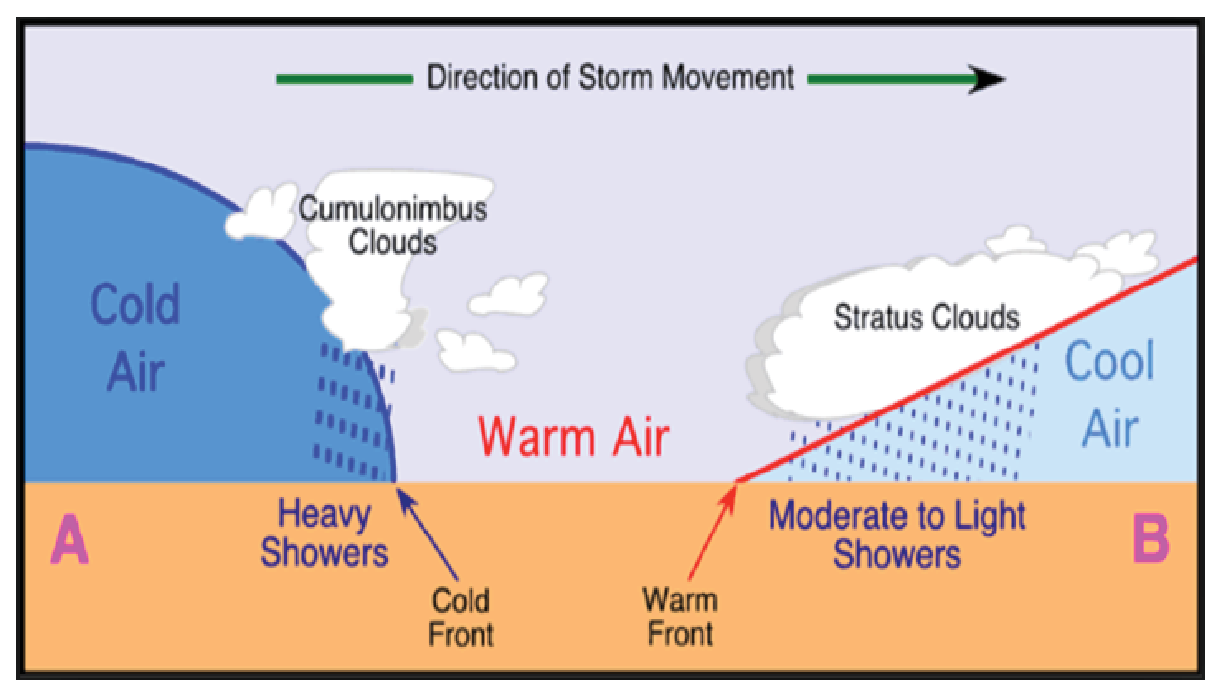
\includegraphics[width = 0.6\textwidth]{cold_warm_fronts}
\caption{Basic mechanisms of precipitation - warm moist air uplifted by or into colder air. On the left is a cold front leading to convective lift and thunderstorms. On the right is a warm front leading to dynamic lift and stratiform rain. Figure from www.physicalgeography.net.}
\label{fig:cold_warm_fronts}
\end{center}
\end{figure}

\section{Measuring Atmospheric Water Vapor}

There are a number of instruments for measuring the amount of water vapor in the atmosphere. These include:

\begin{enumerate}
\item Radiosondes: A radiosonde is a battery powered telemetry instrument package with sensors for sampling various atmospheric variables as it is carried up by a balloon from ground launch to between 20-30 km altitude\footnote{http://www.wrh.noaa.gov/rev/tour/UA/introduction.php}. While radiosondes have the advantage that they can measure the vertical distribution of water vapor, they have the distinct disadvantages that they are typically only launched two times a day (at 0000 and 1200 UTC) and from only a handful of locations (the entire CONUS is covered by a mere 90 radiosonde launch sites).
\item Radiometers. Ground-based water vapor radiometers measure the background microwave radiation emitted by atmospheric water vapor along a given line of site \cite{batelaan1976development}. An advantage of these instruments is their ability to make continuous measurements of water vapor. Disadvantages are cost, calibration, and sparse spatial deployment. They are also limited in that they do not work when it is raining.
\item Satellites. The GOES (Geostationary Operational Environmental Satellite) system provides two sources of information about the water vapor (REFERENCE Forsythe et al.): imagery through its water vapor channel (at 4km spatial resolution, 15 min temporal resolution), and sounder retrievals (at 20km spatial resolution, 1hr temporal resolution). Both of these observations, however, are negatively impacted by cloud cover.
 \item GPS-Meteorology. GPS-meteorology (GPS-Met) is a technique that allows GPS receivers to perform the multiple functions of position estimation and precipitable water vapor estimation \cite{bevis1992gps}. For a given GPS receiver, precipitable water vapor estimates can be made with 30-minute temporal resolution. In regions, such as the middle and western U.S., where there is a high density of Continuously Operated GPS Reference Stations (CORS), techniques have been developed to combine the water vapor measurements from multiple stations into 2D and 3D water vapor fields. The spatial resolution of the field depends on the density of GPS stations (spatial Nyquist). While GPS-Met cannot provide the spatial and temporal resolution of satellites, it has the advantage that it is accurate in all weather conditions and not impacted by clouds or precipitation.
\end{enumerate}

Based on our previous work \cite{nagarajan2015lowcost}, where we developed low-cost GPS-Met systems for near real-time Integrated Precipitable Water Vapor (IPW) estimation and an infrastructure for disseminating the IPW data on-line, we will use the GPS-Met technique as our source of atmospheric water vapor information.\footnote{UMass operates two low-cost GPS-Met stations in the Dallas-Fort-Worth, Texas metroplex region, one (site designation CNVL) at the Univ. of Texas at Arlington and another (site designation NWSD) at the NWS Dallas-Fort-Worth Weather Forecast Office (WFO). IPW observations from these two sites is published on-line at http://emmy9.casa.umass.edu/gpsmet/2015/).

\subsection{GPS Meteorology Technique}

The Global Positioning System (GPS) is a system of satellites operated by the U.S. Department of Defense (DoD). First launched in the 1970s for the purpose of military navigation, the system was later opened up for civilian use. The GPS system consists of a core of 24 satellites flying at 22,200 ft AGL orbiting in 6 different orbital planes inclined at $55^{\circ}$ to each other \footnote{http://www.gps.gov/systems/gps/space/}. For a GPS receiver located in the CONUS the number of satellites in view at any one time ranges between 8 and 12, though only 4 are required for an estimate of horizontal and vertical position.

The signal path from a given satellite to a GPS receiver is called a slant path. Since GPS satellites are not in geosynchronous orbit, the azimuth and elevation angles of the slant paths to the satellites in view change with time, as does the particular set of satellites in view (see the animation at https://en.wikipedia.org/wiki/Global_Positioning_System). Along each slant path a GPS receiver receives carrier signals at two distinct frequencies $L_1$ ($f_1 = 1575.42 MHz$) and $L_2$ ($f_2 = 1227.60 MHz$). These carrier signals are modulated as a sequence of bits called Pseudo Random Noise (PRN) and each satellite is identified by a unique PRN code \cite{hoffman2008gnss}. From the carrier signals (code and carrier phase) the GPS receiver obtains measurements of the distance (pseudorange) between the satellite and the receiver. As the GPS carrier signals travel from a satellite to a receiver, they accumulate delays that cause the pseudoranges to accumulate errors,

\begin{equation}
P_r^s(t_{r})  = \rho_r^s - (\delta t_r - \delta t^s) * c +  \delta_{r,ion}^s + \delta_{r,trop}^s + \xi
\label{eqn:totDel}
\end{equation}

Here $P_r^s$ is the code pseudorange measurement from satellite $s$ to receiver $r$, $\rho_r^s$ is the geometric distance as a function of the receiver and satellite coordinates, and the rest of the terms are range corrections - $delta t^s$ and $delta t_r$ the clock corrections for the satellite and receiver respectively, $c$ is the speed of light in vacuum, $\delta_{r,ion}^s$ is the correction for the signal delay through the electrically charged ionosphere, $\delta_{r,trop}^s$ is the correction for the refractivity induced delays through the troposphere, and $\x$i are residual corrections for things like multipath delay and receiver and satellite hardware biases (cf. \cite{ming2014}).

For the geodest, position accuracy is limited by the accuracy of the clock, ionospheric, and tropospheric corrections. For the meterologist, its the tropospheric correction that is of interest, since the tropospheric delay is the term that varies with atmospheric water vapor content \cite{bevis1992gps} \cite{rocken1995gps} \cite{duan1996gps}. Estimating the tropospheric delay from the observed code range and carrier phase requires estimating and subtracting the other correction terms. For high accuracy, such as required by the GPS-Met application, the so-called double differencing technique is often used \cite{remondi1984using}, \cite{alber2000obtaining}. This involves taking the differences of the pseudorange equations between two receivers and two different satellites and then taking the difference of these differences. If the baseline distance between the two receivers is sufficiently large (> 500 km) that the observables are uncorrelated, then the result of double differencing is the elimination of both satellite and receiver clock errors (the $(\delta t_r - \delta t^s) * c$ term in eq. \ref{eqn:totDel}). For the electrically charged ionosphere, which is the region of the atmosphere between 60 and 1000 km altitude, the ionospheric delay (the $\delta_{r,ion}^s$ term in eq. \ref{eqn:totDel}) is frequency dependent (dispersive) \cite{spilker1980gps}. This delay, which amounts to between 1 and 15 meters of pseudorange error, can be estimated to millimeter precision via linear combinations of the GPS dual frequency observables \cite{rocken1995gps}.\footnote{The lowest cost GPS receivers, such as those in cell-phones, are single frequency receivers that use $L_1$ to estimate position. It is because these receivers cannot correct for the large ionospheric delay as accurately as dual-frequency receivers that they are not generally used for the GPS-Met application.} Residual errors ($\xi$ in eq. \ref{eqn:totDel}), such as due to multipath, are avoided by careful selection of GPS site to avoid obstructions such as cell phone towers and buildings.

What remains after applying the above corrections is the tropospheric delay. The troposphere is the lowest portion of the atmosphere from the earth's surface to about 17 km and is the site of all weather on earth. The excess path length that GPS signals travel in the troposphere is due to refraction and can reach up to 2.5 meters at sea-level. This excess path length is given by \cite{bevis1992gps}, \cite{ming2014},
 
\begin{equation}
\delta_{r,trop}^s = 10^{-6} \int N ds + (S - G)
\end{equation}

where $N$ is the refractivity, $S$ is the actual signal path and $G$ is the geometric signal path respectively along the slant path between satellite $s$ and receiver $r$, and the integral is also evaluated along the slant path. The refractivity, $N$, can be split into a dry part, $N_h$, (refractivity of dry air) and a wet part, $N_w$, (refractivity due to water vapor) \cite{davis1985geodesy}, \cite{saastamoinen1972atmospheric},

\begin{equation}
\delta_{r,trop}^s = 10^{-6} \int (N_h + N_w) ds + (S - G)
\end{equation}

The refractivities depend on pressure, temperature, and humidity according to,

\begin{equation}
N_h = 77.6 (\dfrac{P_d}{T}), N_w = 64.8 (\dfrac{P_w}{T}) + 3.776 \cdot 10^{5} (\dfrac{P_w}{T^2})
\end{equation}

where $P_d$ and $P_w$ are the partial pressures (in millibars) of dry air and water vapor respectively, and $T$ is the surface temperature (in degrees Kelvin).

A GPS-Met estimation of the right hand side of the equation for tropospheric delay proceeds as follows. The tropospheric delay along a slant path is called the Slant Total Delay (STD). This is broken into a Slant Hydrostatic Delay (SHD) term and a Slant Wet Delay (SWD) term,

\begin{equation}
STD = SHD + SWD
\end{equation}

Of these, the SHD accounts for the majority of the excess path length, or about 2 meters, while the SWD accounts for only about 1-2 meters of excess path length. The STD is commonly written in terms of the hydrostatic and wet delays in the zenith direction as (cf.\cite{duan1996gps}),

\begin{equation}
STD = m_h(\theta) ZHD + m_w(\theta) ZWD
\end{equation}

where $m_h(\theta)$ and $m_w(\theta)$ are mapping functions (inversely proportional to the sine of the slant path elevation angle $\theta$) for the hydrostatic and wet components respectively. For elevation angles above $15^{\circ}$ the hydrostatic and wet mapping functions are essentially equal allowing us to write,

\begin{equation}
\begin{align*}
STD &= m_n(\theta) ZHD + m_n(\theta) ZWD \\
&= m_n(\theta) ( ZHD + ZWD ) \\
&= m_n(\theta) ZTD
\end{align*}
\end{equation}

where,

\begin{equation}
ZTD = ZHD + ZWD
\end{equation}

is the Zenith Total Delay. The ZTD is determined from the STDs \cite{tralli1990stochastic} and the ZWD is determined as,

\begin{equation}
ZWD = ZTD - ZHD
\end{equation}

where the ZHD is a slowly varying quantity that can be estimated to a fraction of a millimeter via the so-called Saastamoinen model \cite{saastamoinen1972atmospheric},

\begin{equation}
ZHD = \dfrac{0.00227768 P_0}{1 - 0.00266 cos(2\phi) - 0.00028 h_{ref}}
\end{equation}

where $P_0$ is the surface pressure (in millibars), $h_{ref}$ is the geodic height of the station (in meters) and $\phi$ is the station latitude. Given the ZWD, the Integrated Precipitable Water (IPW), which represents the depth of water in mm per square meter that the column of atmosphere directly over the GPS receiver is holding in the vapor state, is given by \cite{bevis1994gps},

\begin{equation}
IPW = \Pi ZWD
\end{equation}

where,

\begin{equation}
PI = \dfrac{10^6}{461,525 ( \dfrac{373,900}{T_m} + 22.1 )}
\end{equation}

and

\begin{equation}
T_m = 70.2 + 0.72 T_0
\end{equation}

with $T_0$ the surface temperature at the GPS receiver location.

\subsection{GAMIT Software}

There are a number of available software packages that one can use for IPW estimation. The one we use in this work is the GAMIT is a software package developed at MIT \cite{herring2015gamit}. In addition to providing high-precision position analysis, GAMIT has routines for GPS-Met IPW estimation. The routines use the double differencing technique and tropospheric delay models described previously.

Inputs to GAMIT are RINEX (Receiver Independent Exchange Format \cite{gurtner2007rinex}) navigation files containing the receiver and satellite clock offsets, observation files containing the code and carrier phase measurements for each slant path at 30 second sample rate, and for the GPS-Met application meteorological files (from a collocated or nearby weather station) containing the surface pressure, temperature, and relative humidity data at the GPS site location. The satellite orbital parameters giving precise orbit information for each satellite are also an input. These are generated by the IGS (International GNSS services) \cite{dow2009international} and are automatically downloaded by GAMIT for the analysis time period in order to correct for orbit errors. Reference stations with baselines of more than 500 km from the GPS stations at which IPW is desired are chosen to satisfy the double-differencing uncorrelatedness requirement \cite{rocken1995gps}. GPS-Met software, such as GAMIT, has been validated to produce precipitable water vapor measurements of better than 2 mm RMS \cite{duan1996gps}.

\subsection{IPW Normalization}

The GAMIT software produces point estimates of IPW. To obtain the spatial distribution of IPW, we need to combine IPW values from multiple GPS receivers. Before we can do so, however, we first need to normalize the IPW values from the different GPS stations. IPW is the amount of water vapor in a vertical column over the site. Because the amount of water vapor the atmosphere can hold is a function of temperature and temperature generally decreases with altitude, IPW will consequently also depend on the altitude of the station. Since IPW depends on temperature, IPW will also change with season so that an IPW value corresponding to low humidity at summer temperatures might be saturated at winter temperatures. Moreover, IPW by itself does not tell the level of saturation, since again that depends on the daily temperature. To account for station height differences, seasonal (monthly) variations, and to identify anomalously high or low IPW values, we normalize the IPW values by the monthly mean and standard deviation before we combine them as follows,

\begin{equation}
NIPW_{ij} = \dfrac{IPW - \mu_{ij}}{\sigma_{ij}} \ \forall \ i,j
\end{equation}

Here the subscripts $i$ and $j$ are for the station and month respectively and $\mu_{ij}$ and $\sigma_{ij}$ are the mean and standard deviations respectively. In the literature NIPW is termed the standardized anomaly of precipitable water vapor and is a common way of presenting precipitable water information \cite{grumm2001standardized}.

\subsection{Multiquadric Interpolation}

To obtain the spatial distribution NIPW we interpolate from a set of point measurements. The paper \cite{tabios1985comparative} describes a number of methods for interpolating geophysical data. The method we chose is the multiquadric method. This method was chosen because it has been shown to perform nearly as well as the more common Kringing technique \cite{radhakrishna2015precipitable} but without the need for historical data.

Similar to Kringing, the multiquadric method is a weighted linear interpolation method where the estimate $h_0$ for any grid point $(x_0,y_0)$ is given by,

\begin{equation}
h_0 = \sum_{j=1}^{n} w_j \cdot h_j
\end{equation}

where $h_j$ is the observed NIPW at point $(x_j,y_j)$ and $w_j$ is the weight giving the influence of $h_j$ in determining $h_0$.

In the multiquadric method the weights $w_j$ are calculated from the matrix of distances between the observed points $(x_j,y_j)$ and the distances between the interpolated point and each observed point as follows. We start by expressing the observed points as a weighted linear combination of the distances between the observations points,

\begin{equation}
h_j = \sum_{i=1}^{n} c_i \cdot d_{ji} \ \forall j = 1,2..n
\end{equation}

where $d_{ij}$ is the distance between GPS site $i$ and GPS site $j$. The coefficients $c_i$ are then determined by,

\begin{equation}
c_i = \sum_{j=1}^{n} \delta_{ij} \cdot h_j \ \forall i = 1..n
\end{equation}

where $\delta_{ij}$ is an element of the inverse of the $n \times n$ distance matrix $d_{ij}, j = 1..n \ and \ i = 1..n$. Given the $c_i$ we can thus write,

\begin{equation}
\begin{align*}
h_0 &= \sum_{i=1}^n c_i \cdot d_{0i} \\
&= \sum_{i=1}^n [ \sum_{j=1}^n \delta_{ij} \cdot h_j ] \cdot d_{0i} \\
&= \sum_{j=1}^n [ \sum_{i=1}^n \delta_{ij} \cdot d_{0i} ] \cdot h_j \\
\end{align*}
\end{equation}

or

\begin{equation}
w_j = \sum_{i=1}^n \delta_{ij} \cdot d_{0i}
\end{equation}

\subsection{IPW Field Generation}

In light of the above discussion, we can summarize our method for obtaining fields of NIPW as follows. Every 30-minutes we do the following,

\begin{enumerate}
\item Obtain GPS navigation and observation files from $N$ GPS sites distributed throughout the geographical region of interest;
\item Obtain Pressure(P), Temperature(T), Relative Humidity(RH) for each GPS station;
\item Put the P, T, RH data in the required RINEX format;
\item Feed the GPS and meterological RINEX files into GAMIT to get IPW values for each station for the current 30-minute interval;
\item Normalize the IPW values based on the average and standard deviation for the given station and given month;
\item Apply multiquadric interpolation to obtain the NIPW field for the current 30-minute interval.
\end{enumerate}

\section{Measuring Rainfall}

The primary instrument for obtaining spatial-temporal fields of precipitation is the ground-based weather radar. There are a number of different weather radar systems in operation in the U.S. These include the 160 long-range WSR-88D, Next Generation Weather Radars (NEXRAD) operated by the U.S. National Weather Service (NWS) for real-time weather monitoring and short-term forecasting and the 45 Terminal Doppler Weather Radars (TDWR) operated by the NWS to provide high-update rate, high-resolution weather and wind data at key major airports. In addition to these, increasing numbers of television stations have their own weather radars, and there are a variety of research weather radars, such as the network of small X-band radars operated by the University of Massachusetts, Center for Collaborative Adaptive Sensing of the Atmosphere (CASA) in the Dallas-Fort-Worth metroplex region.

As a weather radar rotates in azimuth, it sends out a narrow, pencil beam of microwave pulse energy and then samples the return echo. This partitions the space around the radar into resolution volumes or voxels (volume elements). Voxels have the shape of a disk on its side: the diameter of the disk determined by the radar's beamwidth; the thickness by the radar's gate spacing. The size $V$ of a voxel in cubic meters thus varies with the square of the range from the radar according to,

\begin{equation}
V = G \cdot \pi \cdot tan^{2}(\theta/2) \cdot R^2
\end{equation}

 where $G$ is the gate spacing in meters, $\theta$ is the beam width in radians, and $R$ is the range from the radar to the voxel in meters. For NEXRAD, with its 1 degree beam and 250 meter gate spacing, this leads to voxel with volumes that are roughly 6 million cubic meters at 10 km from the radar to 3 billion cubic meters at the radar's maximum (Doppler) range of 230 km.

Under assumptions that the voxels are completely filled with liquid hydrometeors (raindrops) and that the hydrometeors are small relative to the radar's wavelength (Rayleigh scattering), weather radars measure the echo from each voxel to infer properties of the hydrometers in the voxel (their density, size, radial (Doppler) motion, (Polarimetric) shape asymmetry, and so on) \cite{bringi2001polarimetric} \cite{doviak1993doppler}. To sample the complete volume around the radar, multiple 360 degree sweeps in azimuth are performed, each at a different elevation tilt angle. Each such 360 degree sweep is termed a Plan Position Indication (PPI) scan, and the sequence PPIs starting at the radar's lowest elevation tilt angle and working up to the radar's highest tilt angle that are performed to cover the volume is called the Volume Coverage Pattern (VCP). The NEXRAD lowest elevation tilt angle is 0.5 degrees, and the standard convective weather VCP has a temporal update rate of approximately 5-minutes between updates of the 0.5 degree lowest elevation PPI.

The main weather radar product, reflectivity ($Z$ in $mm^6/m^3$), is defined as the 6-th moment of the drop size distribution \cite{doviak1993doppler}. 

\begin{equation}
Z = \int_{0}^{\infty} N(D) D^6 dD
\label{eqn:reflectivityDef}
\end{equation}

 where $D$ is the (volume equivalent spherical) drop size (diameter in mm) and $N(D)$ is the drop size distribution given by (Marshall-Palmer model) \cite{doviak1993doppler}. 

\begin{equation}
N(D) = 8000 \exp (-4.1 R^{-0.21} \Lambda D)
\label{eqn:MarshallPalmer}
\end{equation}

where $R$ is the rain rate (in mm/hr).

Assuming the drop size distribution in \ref{eqn:MarshallPalmerl}, \ref{eqn:reflectivityDef} can be solved to obtain $Z$ in terms of the median drop size $D_{0}$  \cite{doviak1993doppler},

\begin{equation}
 Z = 642 D_{0}^7
\end{equation}

or in terms of rain rate,

\begin{equation}
 Z = 297 R^{1.47}
 \label{eqn:ZRrelationship}
\end{equation}

Given the above relationships, Table \ref{Radar_Table} relates reflectivity (in dBZ = $10 log_{10} Z$) to median drop size $D_{0}$ (in mm) and rain rate $R$ (in mm/hr)\footnote{We remark that the Z-R relationship in equation \ref{eqn:ZRrelationship} is only one of many such relationships. Others include the famous 1948 $Z = 200 R^{1.6}$ Marshall-Palmer relationship \cite{marshall1948distribution} and the $Z = 300 R^{1.4}$ relationship used by the NWS as the default Z-R relationship for the WSR-88D radar network http://www.srh.noaa.gov/tlh/?n=research-zrpaper}. 
%%%%%%%%%%%%%%%%%%%%%%%%%%%%%%%%%%%%%%%%%%%%%%%%%%%%%%
\begin{table}
\begin{center}
\caption{Reflectivity as a function of median drop size diameter and rainfall rate.}
\label{Radar_Table}
\begin{tabular}{|ccc|}
\hline
dBZ &$D_{0}$ (mm) & $R$ (mm/hr) \\
\hline
-42  & 0.1 & - \\
0 & 0.4 &  - \\
10 & 0.6 & 0.1 \\
20 & 0.8 & 0.5 \\
30 & 1.1 & 2.3 \\
40 & 1.5 & 11.0 \\
50 & 2.1 & 52.0 \\
\hline
\end{tabular}
\end{center}
\end{table}
 Noting that cloud droplets average $12 \mu m = 0.012 mm$, and that even
 the high-powered NEXRAD only has -21dBZ sensitivity at 10km
 (estimated from the WSR-88D specification of -7.5 dBZ at 50 km \footnote{https://www.roc.noaa.gov/WSR88D/PublicDocs/NTR96.pdf}
 and the fact that minimum detectable reflectivity is proportional to
 range squared), we see that weather radars generally cannot detect
 clouds or uncondensed water vapor, but can only detect active
 precipitation.
 We also remark that although dual-polarimetric weather radar, such as
 the upgraded NEXRAD, do provide a rainfall rate product \footnote{https://www.ncdc.noaa.gov/data-access/radar-data/nexrad-products}, in this
 thesis we will use reflectivity as a surrogate for rainfall rate
 with ~30dBZ and above indicating rainfall and the dBZ value reflecting
 rainfall intensity.
 Specifically, we will use the NEXRAD 0.5 degree reflectivity PPI product
 as an indicator of precipitation activity and intensity at ground level.\footnote{To say that the 0.5 degree NEXRAD reflectivity product gives the rainfall at ground level ignores the fact that the earth is
 curved while radar beams travel in essentially straight lines leading
 to an increase in radar beam height above ground level with distance from
 the radar. In particular, we are ignoring the fact that even at its
 lowest tilt of 0.5 degrees, the bottom of a NEXRAD beam is some 3000
 meters (10,000 feet) above ground level at the radar's maximum (Doppler)
 range of 230 km.}

\chapter{Data Set}

The data set we will use for our nowcasting experiments comes from the Dallas-Fort-Worth (DFW) region. Part of the infamous U.S. "tornado alley", DFW spring and summer weather is dominated by convective thunderstorms that move in lines generally from west to east through the region. We choose the DFW region because we understand its climatology (through CASA's more than 15 years of operating networks of weather radars in tornado alley, first in Oklahoma and now in DFW) and because the DFW region has a high density of GPS receivers and weather stations whose data are publicly available on-line for our use.

We take as the center of our region the NWS KFWS NEXRAD radar in Fort-Worth Texas.\footnote{http://radar.weather.gov/radar.php?rid=fws} Within the 230 km coverage range of the radar we identified 44 Regional Reference Points, i.e., high performance dual-frequency GPS receivers. These GPS receivers, which are operated by the Texas Dept. of Transportation (TxDOT)\footnote{http://www.txdot.gov/inside-txdot/division/information-technology/gps.html}, were deployed to provide precise position information for Geodetic studies. As such these GPS receivers do not have collocated weather stations. For the weather data (surface temperature, pressure, and relative humidity) required for IPW estimation, we used data from the network of Automated Surface Observation Stations (ASOS) operated by NOAA NWS\footnote{http://www.nws.noaa.gov/asos/}. Figure \ref{fig:GPS_ASOS_Loc} shows the relative locations of the GPS receivers and ASOS stations within the 230 km coverage range of the KFWS radar. Table \ref{table:GPS_ASOS_table} in Appendix A gives the locations and heights of the the GPS receivers and ASOS weather stations.

\begin{figure}[!t]
\begin{center}
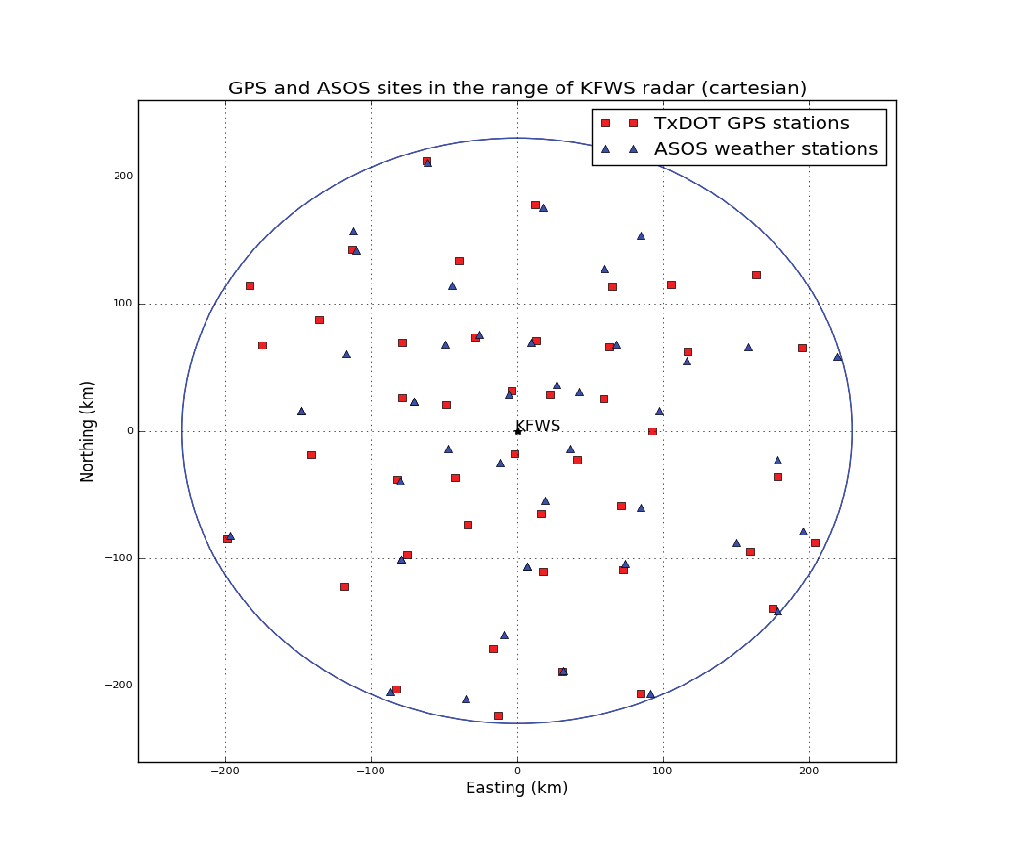
\includegraphics[width = 0.8\textwidth]{GPS_ASOS_Locations}
\caption{GPS and ASOS stations within the KFWS 230 km coverage range.}
\label{fig:GPS_ASOS_Loc}
\end{center}
\end{figure}

GPS RINEX files of code range and carrier phase for the entire year of 2014 were downloaded for each of the 44 stations from databases maintained by SOPAC\footnote{http://sopac.ucsd.edu/} \cite{bock1997scripps} and CORS\footnote{http://www.ngs.noaa.gov/}\cite{snay2008continuously}. The meteorological data from the ASOS stations were obtained at 30 minute intervals for the year of 2014 from Teresa Vanhove of UCAR\footnote{http://www.suominet.ucar.edu/}. The KFWS 0.5 degree reflectivity product for the entirety of 2014 was downloaded from NCDC\footnote{https://www.ncdc.noaa.gov/data-access/radar-data}. For the long baseline stations needed for double differencing, we chose the four stations: AC20 in Girdwood Alaska, CONZ in Concepcion Chile, P019 in Fairfield, Idaho, and UNBJ at the University of New Brunswick, Canada. The closest of these stations, P019 is approximately 1500 km from the KFWS radar defining the center of the DFW GPS network. These stations were chosen to ensure that there was always at least one satellite that had a view of all of the TxDOT GPS stations and one of the baseline stations.

To get the meteorological data for a particular TxDOT GPS station, we found the closest ASOS site and used the equations from \cite{bai2003gps} to interpolate the surface temperature (T), pressure (P), and relative humidity (RH) data from the MSL height of ASOS site to the MSL height of the GPS station,
 
\begin{equation}
P_{SL} = P_{MSL} \cdot (1 - 2.26 \cdot 10^{-5} \cdot H)^{5.225}
\end{equation}
\begin{equation}
T_{SL} = T_{MSL} - 0.0065 \cdot H
\end{equation}
\begin{equation}
RH_{SL} = \dfrac{RH_{MSL}}{e^{-0.0006396 \cdot H}}
\end{equation}

In the above, $P_{SL}$ is the pressure at the station level, $P_{MSL}$ is the pressure at mean sea level, and $H$ is the height of the station (in meters MSL). We then wrote a Python script to mine the large database of met values from the various ASOS sites to generate the met RINEX files for each GPS station in 30-minute intervals. 

The GPS and met RINEX files for each station were run through GAMIT to produce 30-minute estimates of IPW for each station for the entire year of 2014. The mean and standard deviation of IPW for GPS station were calculated for each month, and the IPW values normalized to obtain the standardized anomaly of precipitable water, which we have denoted NIPW. The NIPW values were then mapped to a 300 km by 300 km, 3km resolution grid centered on the KFWS radar using multiquadric interpolation method.

The data processing was done on a Ubuntu server where GAMIT is installed. The server has 16 CPUs with 4 cores each. The data processing was performed in a manner that optimized the computation resources of the server thus allowing many days to be processed at the same time. Specifically, the 44 GPS stations were also broken down into 4 sub-networks that we processed simultaneously. Because we used the double differencing approach the stations had to be processed in pairs consisting of the station and its long-baseline reference.

Regarding the NEXRAD reflectivity data, this was first down-sampled from its native ~5-minute update rate to the 30-minute NIPW update interval. We then performed a polar to Cartesian coordinate conversion to map the reflectivity field to the same 3 km grid resolution as used for NIPW. The result is two fields of 10,000 pixels each updated every 30-minutes, one of NIPW (a measure of atmospheric water vapor) the other of reflectivity (a measure of rainfall).

\section{Experimental Data Set}

Machine learning involves first training the machine learning system on a training data set and then testing it on a separate validation data set. For our training and validation sets, 23 days from 2014 were chosen. These days were selected from the months of May, July, and August as it is during these months that strong convective storms are most likely. From these months, the days chosen were what we termed "weather anomaly" days, where a day is a weather anomaly day if 30 or more of the 44 GPS sites had NIPW values that exceeded 2 standard deviations from the mean during any 30-minute interval. Table \ref{table:weather anomaly} lists the 23 days comprising our training and validation sets.

\begin{table}
\begin{center}
\caption{Weather anomaly days}
\begin{tabular}{ |c|c|c| } 
 \hline
 May & July & August  \\ 
 \hline
 08 & 15 & 11 \\ 
 09 & 16 & 16 \\
 12 & 17 & 17 \\
 13 & 18 & 18 \\
 23 & 28 & 19 \\
 24 & 29 & 29 \\
 25 & 30 &      \\
 26 & 31 &      \\
 31 &     &       \\
\hline
\end{tabular}
\label{table:weather anomaly}
\end{center}
\end{table}

\section{Preliminary Data Analysis}

To give a sense of typical IPW values in the DFW region and how these IPW values vary with height, Figure \ref{fig:Highest_Lowest_Site} plots the monthly means for the 4 highest and 4 lowest GPS sites. Clear in the plot is the height dependence, with mean IPW inversely proportional to station height.

To see how IPW varies with season in the DFW region, Figure \ref{fig:IPW_site_dist} plots histograms of the IPW values observed at the highest (TXBX) and lowest (TXC3) GPS sites. Clear in the histograms is the seasonal dependence with higher mean IPW values during the warmer months (April-September) and lower mean IPW values during the cooler months (October-March). Again we see the height dependence with the IPW of the highest station having generally lower IPW values than the lowest station. REMEMBER TO PUT THE MEANS AND STDS ON THE PLOTS.

These first two plots illustrate why IPW values are typically normalized before they are combined to produce a field. Our approach of normalizing to obtain the number of standard deviations from the mean removes height and seasonal differences and also allows us to infer something about saturation level as many standard deviations above (below) the mean will typically indicate a saturated (dry) atmosphere respectively without a need to estimate relative humidities or dew points.

Finally, to see visually if there are any spatial and temporal correlations between NIPW and reflectivity that might allow a machine learning algorithm to predict rain, Figure \ref{fig:ipw_radar} shows the reflectivity fields superimposed atop the NIPW fields for three different storm cases from our experimental data set. These storm cases include May 8th (left hand column), July 17th (middle column), and August 29th (right hand column). Going from the top to the bottom of each column, the fields show the joint evolution of reflectivity and NIPW in 30 minute time intervals.

The May 8th and August 29th cases show lines of thunderstorms moving through the DFW region. In both these cases, we can clearly see that the reflectivity seems to ride just slightly behind the moving ridge of high NIPW. For the July 17th case, which is more of a slow moving stratiform event, the reflectivity surrounds a very slow moving peak of NIPW. Thus, whereas it might be difficult to predict the rainfall at a given location from reflectivity alone, noting that rainfall tends to track just behind large peaks in NIPW can be expected to aid rainfall nowcast ability. We explore this conjecture in the next chapter.

\begin{figure}[!t]
\begin{center}
\includegraphics[width = 0.7\textwidth]{Highest_Lowest_Site}
\caption{Mean IPW for each month for 4 highest and 4 lowest stations. The height is measured as the Geodic height in meters.}
\label{fig:Highest_Lowest_Site}
\end{center}
\end{figure}

\begin{figure}[!t]
\begin{center}
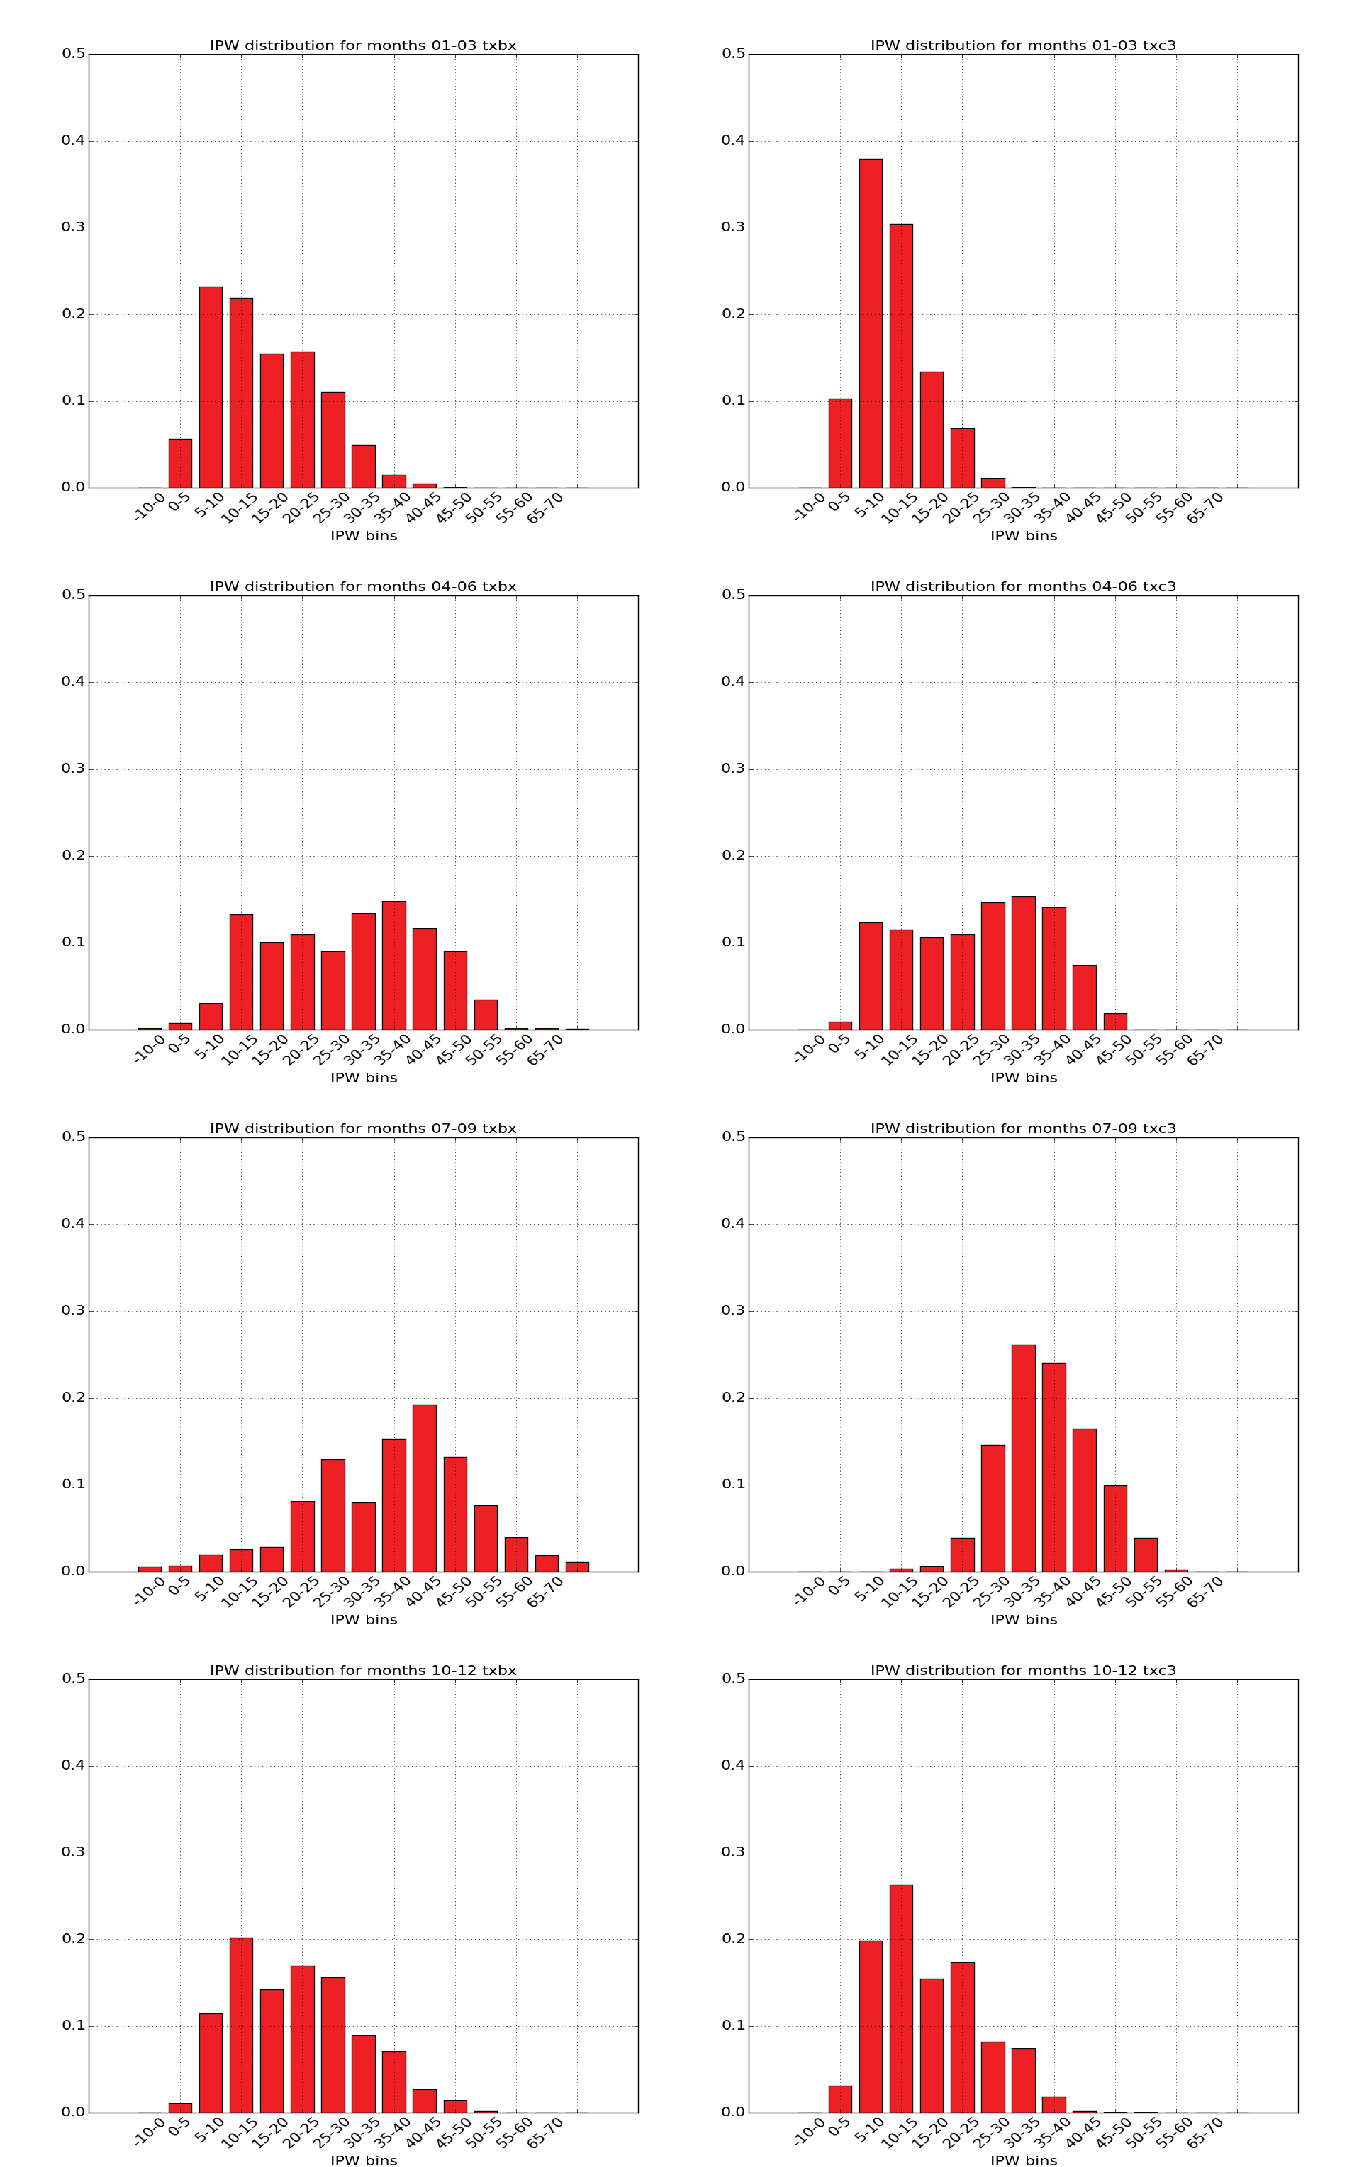
\includegraphics[width = 16cm,height = 20cm]{IPW_site_dist}
\caption{IPW histograms for each season for the highest station TXBX (left) and lowest station TXC3 (right).}
\label{fig:IPW_site_dist}
\end{center}
\end{figure}

\begin{figure}[!h]
\begin{center}
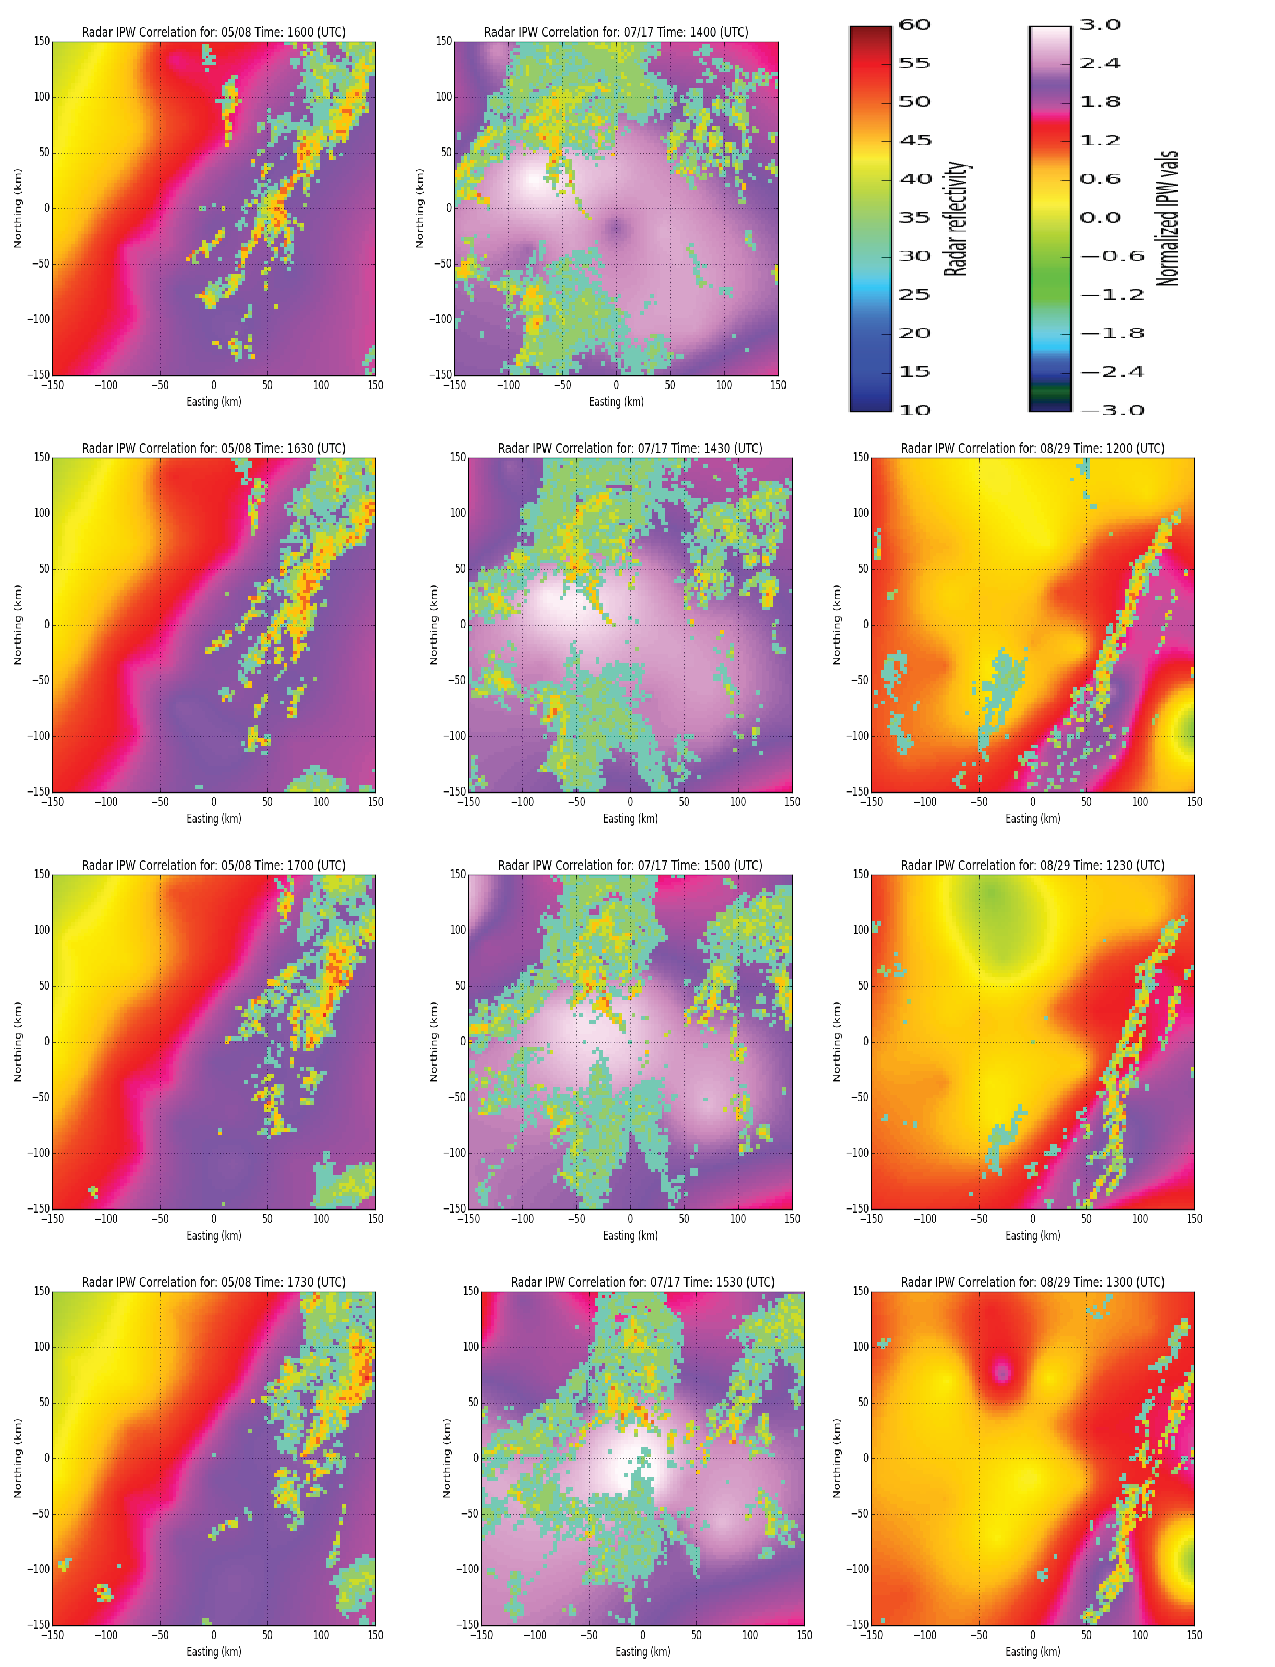
\includegraphics[width = 15cm,height = 20cm]{RadarIPWProposal}
\caption{Reflectivity fields overlayd onto IPW fields for three storms left: May 8th, center: July 17th and right: August 29th)}\label{fig:ipw_radar}
\end{center}
\end{figure}

\chapter{Initial Learning Results}

For our initial machine learning results we chose to apply machine learning techniques similar to those used in \cite{mecikalski2015probabilistic}. The problem they looked at was similar to ours in that they were trying to predict convective initiation 0-60 minutes in advance using GOES-R satellite data and NWP data. For their predictions they used two different machine learning classifiers, logistic regression and random forests. The accuracy of predicting convective initiation one hour in advance was reported as 84 \% and 71\% for logistic regression and random forest respectively.

\section{Problem Setup}

The classifiers we choose for our initial machine learning experiments were the Naive Bayes classifier and the Random Forest classifier. Our goal is to make a binary 0, 1 (no rain, rain) prediction 1 hour in the future for a random subset of the 10,000 pixels that make up the 300 square km grid around the KFWS radar, where rain is taken as a pixel reflectivity value exceeding 24 dBZ.

With $y\in[0,1]$ as the dependent binary variable indicating "rain" and "no rain" at a pixel point, the feature set for determining the dependent variable $y$ is chosen to be the most recent four frames (most recent 2 hours) of NIPW and reflectivity fields. Specifically, the feature set for predicting rain at a given pixel was determined from the four most recent fields of NIPW and reflectivity in the 33 by 33 pixel subgrid centered on the pixel. As a simplification, we averaged the NIPW and reflectivities in each 33 by 33 grid. Our initial learning problem is thus one of making a binary rain, no-rain prediction of the state of the center pixel 1-hour in the future from a feature set consisting of the averages of the NIPW values and reflectivities in the most recent 4 frames (past 2 hours) in the 33 by 33 (100 by 100 km) region surrounding the pixel. As shown in PUT A FIGURE SHOWING THE PIXEL POINTS, we do this for a total of PUT NUMBER OF PIXELS HERE pixel locations uniformly distributed throughout the 10,000 pixel DFW domain.

\section{Training and Validation}

The experimental set (see Section 3) was broken down into a series of training set and validation sets using the K-Fold cross validation technique with $k=7$ \cite{friedman2001elements}. The algorithm for cross validation technique is explained as follows:
 
\begin{enumerate}
\item Randomly shuffle the experimental data set. 
\item Divide the experimental data set into K equal parts.
\item Train on K-1 of the blocks and test on the remaining block. 
\item Repeat until all K blocks have been tested on using the other K-1 blocks as training examples. 
\end{enumerate}

\section{The Naive Bayes Classifier }

The Naive Bayes or Bayes optimal classifier \cite{zhang2004optimality} is based on the assumption that each variable behaves independently with respect to the other variables and disregards any correlation one variable may have on any other. Given a training example $x_i \in \mathbb{R}^D$ and its corresponding output $Y_i = c$ where $c \in G$ where $G$ is the set of all possible classes, we can compute the prior probability $P(Y = c) = \pi_c$ and the true probability $\phi_c(x) = p(X = x | Y = c)$.  We can then apply Bayes rule to calculate the posterior probabilities,

\begin{equation}
P(Y = c | X = x) = \dfrac{\phi_c(x) \pi_c}{\sum_{c' \in Y}\phi_{c'}(x) \pi_{c'}}
\end{equation}

Making the "Naive" assumption that all variables are independent we can say that,

\begin{equation}
\phi_c(x) = p(X = x | Y = c) = \prod_{d=1}^{D} p(X_d = x_d | Y = c) = \prod_{d=1}^{D}\phi_{cd}(x_d)
\end{equation}

Thus we can write the general classification function as,

\begin{equation}
f_{NB}(x) = \operatornamewithlimits{argmax}\limits_{c \in Y} \pi_c \prod_{d = 1}^{D} \phi_{cd}(x_d)
\end{equation}

The Naive Bayes classifier despite making its fundamental assumption of independent variables, which is never true for real-world problems, is capable of forming complex decision boundaries.

\section{Random Forest Classifier}

The random forest classifier consists of an ensemble of CART (Classification and Regression Trees) where the decision on deciding the class variable is made via majority vote of an ensemble of decorrelated decision trees in the forest \cite{breiman2001random}. Trees are ideal candidates for random forests as they can capture complex interactions in the data.

A simple decision tree works on the principle of finding a best split amongst all variables $d \in D$ given a set of training vector/output pairs $(x,y)$ where $x$ is a vector with dimension $D$. Classification is based on finding a threshold $t$ such that a variable in a data case $x_d$ is split based in $x_d < t \ or \ x_d > t or \ x_d =t$. The data case is assigned to the left or right branch of the tree based on $x_d$ and threshold $t$. The data cases are traversed through the tree from the root node to the leaf of the tree and the class is determined at the leaf.

As a decision tree learns, finds both the optimal variable $d$ to split on and the optimal threshold value $t$ using a greedy heuristic that tries to maximize the training accuracy. In a geometrical sense the decision tree breaks the $D$ dimensional feature space into smaller regions such that each region contains the maximum number of instances that belong to a single class. Hence a fundamental metric $p_{km}$ is the proportion of observations in the m-th region that are in the k-th class. This leads to the so-called "Genie Index" criterion,

\begin{equation}
C_{GI} =  \sum_{k=1}^{K} p_{km} (1 - p_{km})
\end{equation}

which decision tree learning seeks to maximize by adjusting the tree parameters $d$ and $t$. Hyperparameters to the algorithm include the number of trees in the forest $B$ and the maximum tree depth. FOR OUR EXPERIMENTS THESE WERE CHOSEN BY A SYSTEMATIC SEARCH PROCESS.
 
The random forest algorithm thus can be summarized by the following algorithm from \cite{friedman2001elements},
 
\begin{enumerate}
\item Initialize the number of trees B in the forest. 
\item for b = 1:B
\begin{enumerate}
\item Draw a bootstrap sample Z of size N examples from the training data
\item Grow a random forest tree $T_b$ to the bootstraped data by recursively repeating the following steps
\begin{enumerate}
\item select m at random from D (ideally $m = \sqrt{|D|}$)
\item pick the best variable split among the m variables based on the Genie criteria
\item split the node to two daughter nodes
\end{enumerate}
\item The classification is based on the majority votes from B trees. 
\end{enumerate}
\end{enumerate}

The random forest thus forms its "decorrelated" trees by picking a set of random variables $m$ at each iteration of each tree. In this fashion an ensemble of weak learners are built.

 One of the key advantages of the Random Forest classifier is its interpretability through variable importance. The variable importance is an attribute of random forest classifier which measures the relative importance of each variable. This is done by measuring the prediction performance of the "OOB (Out Of Box Samples)". When the $b^{th}$ tree is being constructed, examples apart from its bootstrapped samples are used to measure its predictive performance at a particular split. Different permutations of the variable split are tried and the performance is measured on the OOB samples. The results are accumulated over all trees and the variables which are most important are ranked.
 
\section{Nowcasting Performance Results}

Given the mechanisms of precipitation discussed in Chapter 2 and our initial analysis in Chapter 3, we believe that the combination of NIPW and reflectivity should be more predictive of precipitation than either NIPW or reflectivity alone. To test this hypothesis, three kinds of predictions were made using the two classifiers on each of the 7 training and validation sets. Predictions using only NIPW fields, predictions using only reflectivity fields, and predictions using both NIPW and reflectivity fields. 

The output of the Bayes and Random Forest classifiers are real numbers between 0 and 1. These can be interpreted as beliefs that it is raining or not raining at a selected pixel location. The actual rain, no-rain decision is determined by a decision threshold - rain if the output exceeds the decision threshold, no-rain otherwise.

A common way to assess the performance of binary classifiers is the Receiver Operating Characteristic (ROC). An ROC plots the probability of correct classification (also called the probability of detection, POD) against the probability of incorrect classification (or probability of false alarm, PFA) as a function of the decision threshold. A good classifier is generally taken as one whose ROC curve is bent towards the (0,1) point (low PFA, high POD). Such a classifier would tend to have a large area under the curve. Figure \ref{fig:ROC_Curves} shows the ROC curves for the two classifiers along with their respective area under the curves. Though the combination of NIPW and reflectivity has a slight performance edge, the ROC curves suggest the combination offers only slight advantage over NIPW or reflectivity alone.

\begin{figure}[!t]
\begin{center}
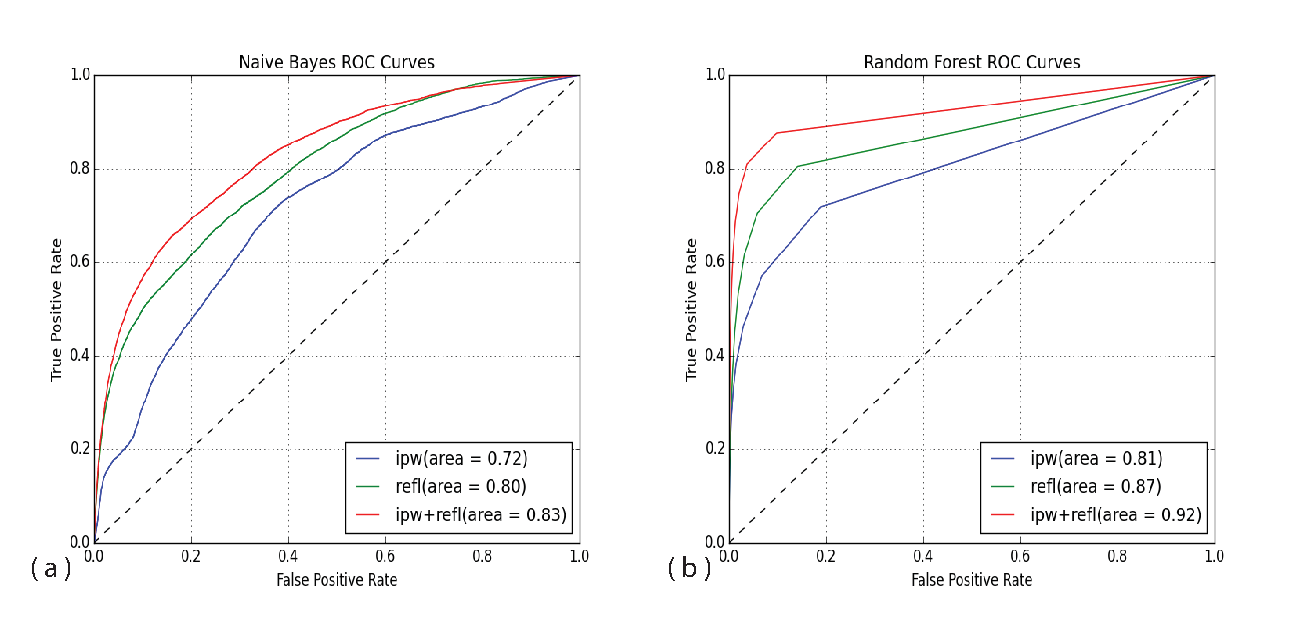
\includegraphics[width = 15cm,height = 9cm]{RF_NB_ROC}
\caption{Receiver Operating Characteristic (ROC) curves for the Naive Bayes precipitation nowcaster (a) and Random Forest precipitation nowcaster (b).}\label{fig:ROC_Curves}
\end{center}
\end{figure}

The high values of area under the ROC curves must not be interpreted as an indication of high performance of the classifiers. This high value is clouded by the fact that there are significantly more no rain cases than rain cases, so that what the high value indicates is merely that we are able to predict the "no rain case" accurately.

What we needed, therefore, was a way of evaluating performance that was better tailored to our problem where we only $~5 \%$ of the experimental data set involved rain cases. The precision-recall curve provides such a solution \cite{powers2011evaluation}. A precision-recall curve starts with the determination of the number of Hits (H), Misses (M), False alarms (F) and Correct negatives (C). From these the precision (P) and recall (R) are defined as follows,
 
\begin{equation}
P = \dfrac{H}{H + F}
\end{equation}

\begin{equation}
R = \dfrac{H}{H + M}
\end{equation}
 
Precision, which is the proportion of cases that are predicted positive that are actually positive, is a measure of confidence. Recall, which is the proportion of real positive cases that are predicted positive, is a measure of sensitivity. A precipitation nowcast system with high recall but low precision may indicate that that the predictor is returning a lot of cases of rain but that only few are actually correct. A system with low recall but high precision indicates that the predictor is returning very few positive results but most of these results are accurate. Ideally a good balance between the two scores is desirable. A measure of this balance is the $f_1$ score, defined as,

\begin{equation}
f_1 = 2 \cdot \dfrac{P \cdot R}{P + R}
\end{equation}

A high value of $f_1$ would indicate a good balance between precision and recall and would thereby indicate that the classifier is making accurate predictions.

Figure \ref{fig:initial_results} shows the precision-recall (P-R) curves for the Bayes and Random Forest classifiers. These are plots of precision vs. recall as a function of the decision threshold. For a P-R curve, best performance is when the curve bends towards the point (1,1). The area under the P-R curve is called the average precision score. Similar to the area under the ROC, a large area under the curve, or large average precision score signifies a good classifier.

\begin{figure}[!t]
\begin{center}
\includegraphics[width = 15cm,height = 10cm]{initial_results}
\caption{Precision-Recall curves for the Bayes precipitation nowcaster (a) and Random Forest precipitation nowcaster (b).}
\label{fig:initial_results}
\end{center}
\end{figure}

In contrast to the ROC which suggested that all of the classifiers gave good performance, here we see a completely different situation. In this case it becomes much more clear that nowcasting using the combination of NIPW and reflectivity performs much better than nowcasting using either one alone, thus confirming our hypothesis. We also see the intuitively appealing result that precipitation nowcasting using reflectivity performs better than precipitation nowcasting using NIPW. This is intuitively appealing since reflectivity is a more direct and immediate measure of precipitation than NIPW.   

What is particularly interesting is how good the ROC results for the Bayes nowcaster are, but how poor its P-R results are. What this seems to show is whereas a classifier that always predicts no rain on a skewed data set that is dominated by no-rain cases can give a good ROC, its poor performance on the few rain cases that do occur will be clearly reflected in the P-R curve. We believe the poor performance of the Bayes classifier is due to the assumption that all of the variables are independent of each other, something that is not true with weather fields which change in smooth continuous ways and for NIPW and reflectivity fields where high NIPW is often followed by high reflectivity (recall Chapter 3). The random forest classifier, which does not make such an assumption performs much better.

The poor performance of the Bayes nowcaster and good performance of the Random Forest nowcaster are further verified by Figure \ref{fig:f1_scores} which plots the $f_1$ scores as a function of the 7 cross-validation training/validation sets. Here the detection threshold was set of 0.5. The random forest classifier has an average $f_1$ score of 0.68 and does not vary much between validation. This suggests that that all all of the misclassified examples are of a very specific type and they are also equally distributed between the validation sets. The Bayes classifier performs poorly ($f_1$ < 0.4) in all cases.

\begin{figure}[!t]
\begin{center}
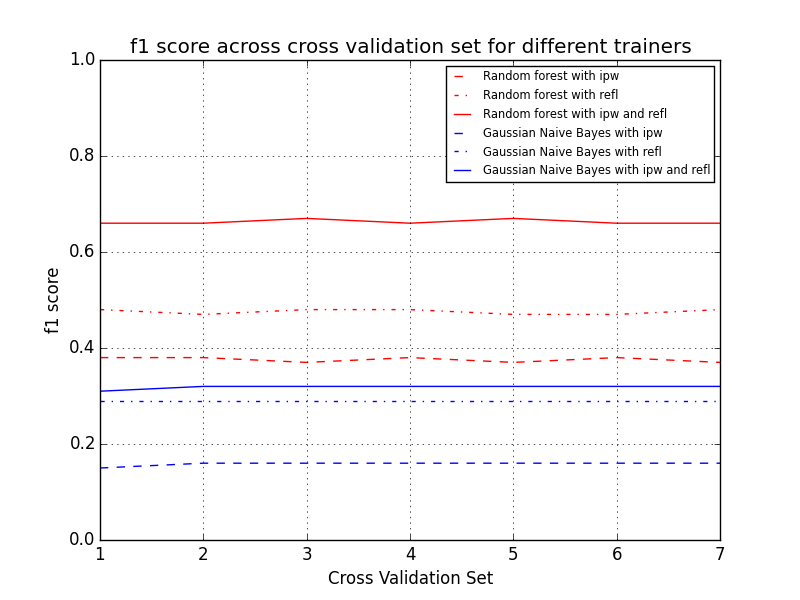
\includegraphics[width = 15cm,height = 9cm]{f1_scores}
\caption{$f_1$ scores as a function of cross-validation training/validation set.}
\label{fig:f1_scores}
\end{center}
\end{figure}

Mentioned earlier was the interpretability of the results learned by a Random Forest classifier through its ability to rank the importance of the different input variables in its decision making. Figure \ref{fig:variable_importance} shows the relative variable importance for the classification done given the input of IPW and reflectivity fields. As seen from the figure, the top 4 most important variables used by the random forest to make its prediction are the oldest and newest IPW and reflectivity fields (i.e., the fields from $t - 2.5$ hours and $t -1$ hours prior to the time $t$ for which the prediction is being made). Again we see the intuitive result that reflectivity is more predictive of precipitation in the short-term than NIPW.

\begin{figure}[!t]
\begin{center}
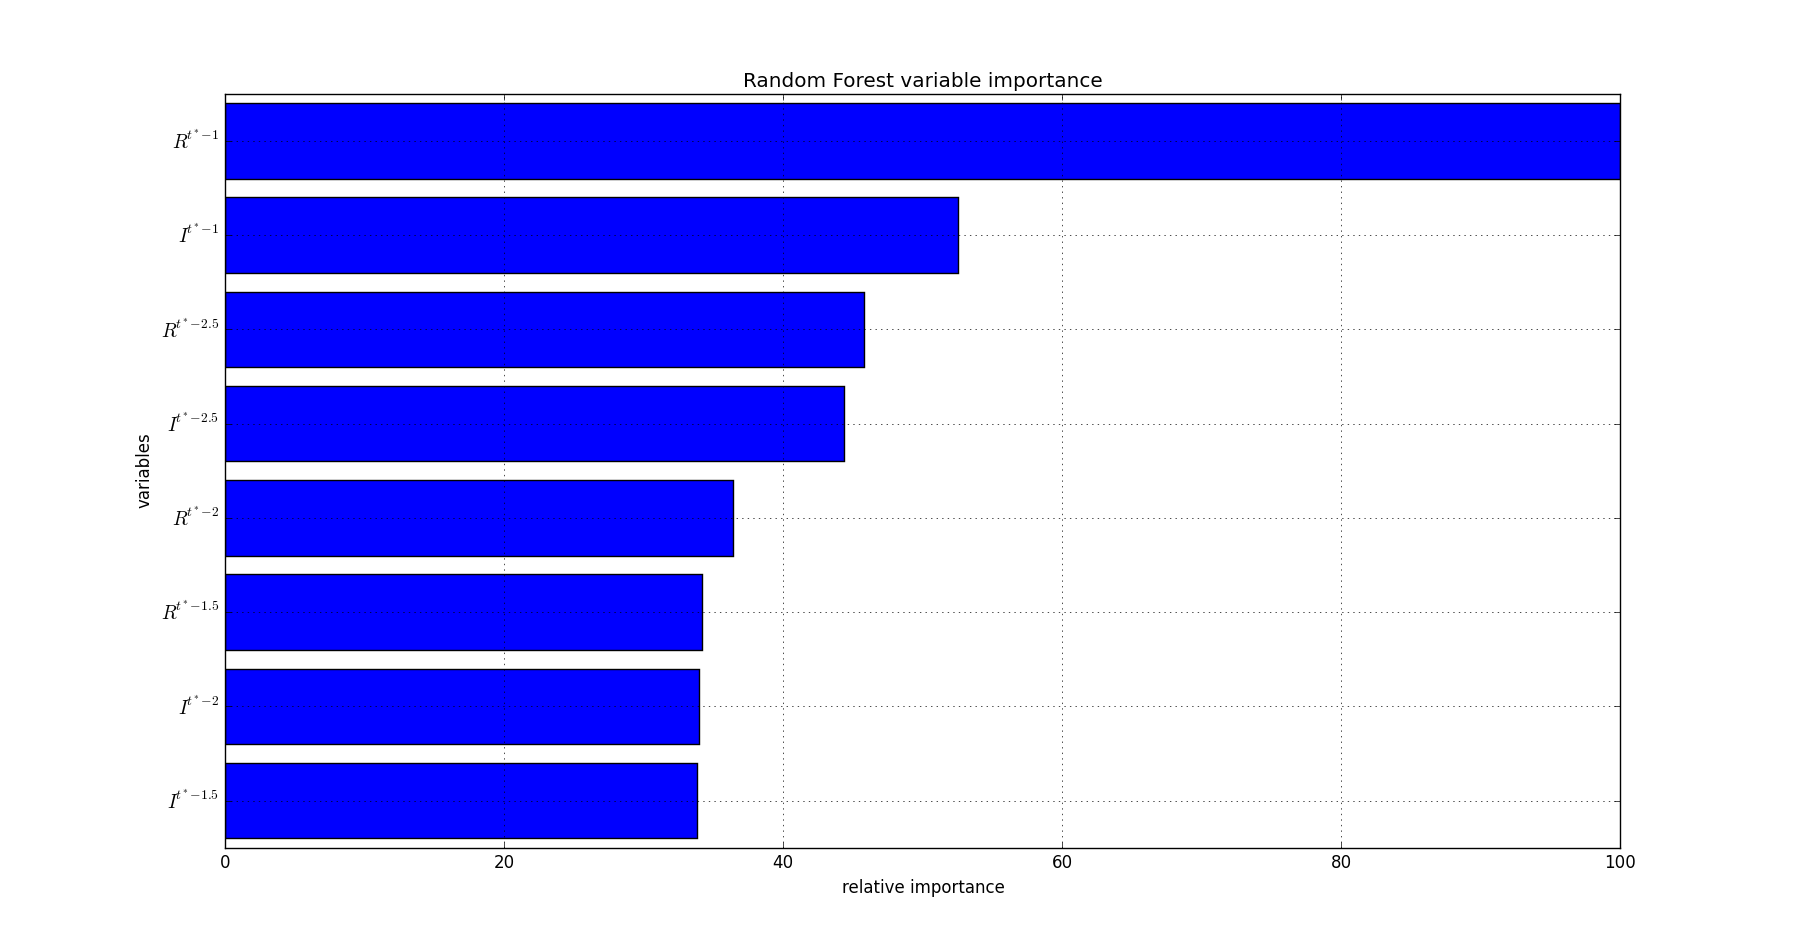
\includegraphics[width = 15cm,height = 12cm]{random_forest_feature_importance}
\caption{Relative variable importance measured by random forest classifier.}\label{fig:variable_importance}
\end{center}
\end{figure}

\chapter{Discussion, Proposed Work, Expected Contributions, and Timeline}

Out of an interest in data science and machine learning, this thesis tackles the challenging problem of nowcasting precipitation from the spatiotemporal evolution of atmospheric water vapor fields (measured by normalized IPW) and rainfall fields (measured by weather radar reflectivity). Following work by \cite{breiman2001random} \cite{mecikalski2015probabilistic}, our initial results applied Naive Bayes and Random Forest classifiers to the problem with mixed results - the Bayes classifier performed poorly, the Random Forest classifier reasonably well.

\section{Proposed Work}

To complete this thesis, we propose to look into other machine learning techniques for finding spatiotemporal patterns in "video" sequences of NIPW and reflectivity.

On reviewing literature for machine learning algorithms that incorporate video sequences as inputs, the paper \cite{shan2007beyond} bears similarity to our problem. In that work the problem addressed was that of recognizing human emotions from two separate video sequences, one focused on the face and the other recording body gestures. In their solution, the authors incorporated a technique from multi-view learning called Canonical Correlation Analysis (CCA). CCA is a method of finding a representation through a basis vector that seeks to maximize the correlation between 2 sets of features \cite{sun2013survey}. In \cite{shan2007beyond} the facial expressions and hand movements were fused using CCA to obtain a set of features which performed better than when the two features were concatenated. The CCA technique has also found success in other problems involving time seres data. The paper \cite{guo2014feature}, for example, examined a stock market data set consisting of historic stock values along with more general economic factors. These two features being correlated and complementary were fused together using the CCA technique to predict the closing price for the stock market the next day using a Support Vector Machine Regressor with a Radial Basis Function Kernel. As one task for our final thesis, we propose to investigate the CCA technique as a way to fuse NIPW and reflectivity fields and to investigate the use of the resulting correlated field of NIPW and reflectivity as an input to a machine learning nowcast algorithm. The CCA technique has been implemented in the Python machine learning package scikit-learn \cite{pedregosa2011scikit}, and can be readily applied to our problem using the two fields.

In addition to the above, we are particularly interested in investigating an application of the so-called deep learning techniques to our problem. Deep learning is a new area of machine learning research at the cutting-edge of artificial intelligence (cf. http://deeplearning.net) that is just recently starting to be applied to the problem of weather forecasting \cite{shi2015convolutional}, \cite{grover2015deep}. We propose to investigate the use of deep learning to not only make a no-rain, rain binary nowcasts, but to try to nowcast rainfall intensity as well. For this effort we propose to use the extensive library of deep learning tools from the Python package Theano \cite{bergstra+al:2010-scipy}. Our plan is to use a GPU instance from Amazon Web Services (AWS) and run our nowcasting experiments in the cloud. This will enable us to try new things and speed up computation significantly.

\section{Expected Contributions}

The expected contributions of this thesis work are as follows: 

\begin{enumerate}
\item A hardware/software design for a low-cost GPS-Met station capable of near-real-time IPW estimates. This work is documented in the publication \cite{nagarajan2015lowcost}.
\item Deployment of two of the low-cost GPS-Met stations that include a high-resolution barometers for the DFW Weather Forecast Office to use for IPW and fine resolution barometric pressure analysis during events such the passing of nearby tornados and other weather anomalies. 
\item A Python-based suite of tools for near-real-time estimates of IPW fields from the network of TxDOT GPS-receivers and NWS ASOS weather stations in the DFW region. This set of tools is capable of automatically downloading the necessary GPS and ASOS data from on-line databases, putting the data in appropriate RINEX formats and directories, executing GAMIT for IPW estimation, and then calling a multiquadric interpolation algorithm to map the results to a field.
\item An improved understanding of the relationships between IPW and precipitation, including the ability to make movies to show visually the joint spatial-temporal evolution of IPW and weather radar reflectivity, and through an analysis of machine-learning techniques such as the Random Forest classifier that can rank the importance of the input variables.
\item Development of Python-based tools analyzing and conducting machine-learning experiments with spatial-temporal fields of weather data that others will be able to use for future weather forecasting and analysis studies.
\item Development, analysis, and comparison of different machine learning approaches for precipitation nowcasting from spatial-temporal sequences of normalized IPW and weather radar reflectivity, including the Naive Bayes classifer, Random Forest classifier, CCA based feature extraction, and deep learning neural network approaches.  
\end{enumerate}

\section{Timeline}

The tentative timeline for completing this thesis is summarized in Table \ref{timeline_table}. 

\begin{table}[!h]
\centering
\caption{Timeline}
\label{timeline_table}
\begin{tabular}{|l|l|l|}
\hline
  & \multicolumn{1}{c|}{Activity}                                                                                         & \multicolumn{1}{c|}{\begin{tabular}[c]{@{}c@{}}Completion \\ Date\end{tabular}} \\ \hline
1 & \begin{tabular}[c]{@{}l@{}}Implementation of a deep learning neural network precipitation nowcast algorithm \\ similar to the one explored in \cite{shi2015convolutional}.\end{tabular} & 01/05/16                                                                        \\ \hline
2 & \begin{tabular}[c]{@{}l@{}}Exploration into the use of the CCA technique for dimensionality \\ reduction, feature extraction and precipitation nowcasting.\end{tabular}                      & 01/05/16                                                                        \\ \hline
3 & Oral presentation of the precipitation nowcasting work at the 2016 Annual Meeting of the American Meteorological Society (AMS) in New Orleans, LA.                                                                                     & 01/12/16                                                                        \\ \hline
4 & Completion of thesis writeup for distribution to committee members. We are also considering the submission of a journal version of the thesis work.                                                                               & 01/30/16                                                                        
\\ \hline
5 & Thesis defense.
\end{tabular}
\end{table}

%\begin{enumerate}
%\item Explore Multi layer Perceptron neural networks and deep learning techniques such as CNN and RNN
%\item Apply CCA technique for dimensionality reduction and see improvements in results
%\item Present results at AMS
%\item Complete write up of above procedures and defend. 
%\end{enumerate}

\appendix
\chapter{DFW PRECIPITABLE WATER VAPOR, REFLECTIVITY NETWORK}

This appendix gives the locations of the sensor assets used for the studies in this thesis.

Weather radar reflectivity data came from the KFWS WSR-88D weather radar located in Fort-Worth, TX (32.569 Deg Lat, -97.299 Deg Lon). This radar defined the center point of our 300 km by 300 km region of study. The table in Figure A.1 gives the locations of the GPS stations used along with the location of the closest ASOS weather station from which the met variables needed for IPW estimation were obtained. 

WE SHOULD ALSO GIVE THE LOCATIONS OF THE LONG-BASELINE STATIONS THAT WERE INCLUDED FOR THE DOUBLE-DIFFERENCING.

AC20 in Girdwood Alaska
CONZ in Concepcion Chile
P019 in Fairfield, Idaho
UNBJ at the University of New Brunswick, Canada.  

\begin{figure}[!h]
\begin{center}
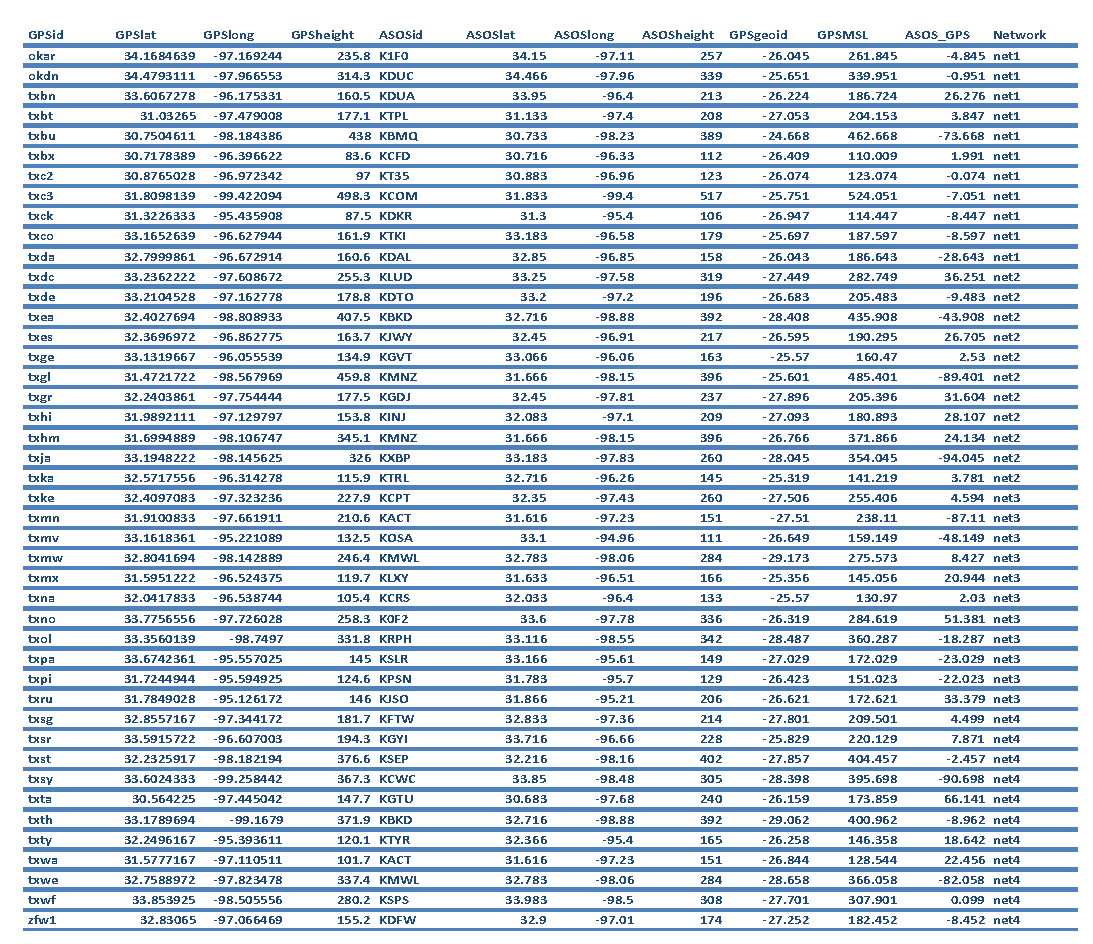
\includegraphics[width = 15cm,height = 16cm]{GPS_ASOS_table}
\caption{GPS ASOS table}\label{table:GPS_ASOS_table}
\end{center}
\end{figure}

\backmatter  %% <--- mandatory


\interlinepenalty=10000  % prevent split bibliography entries
\bibliographystyle{umassthesis}
\bibliography{umthsmpl}
\end{document}

